\chapterimage{chap21.jpg}
\chapter{随机事件和概率}
\begin{definition}[随机试验]
	\begin{itemize}
		\item $\text{试验可以在相同条件下重复进行}$
		\item $\text{试验的所有结果是明确可知道的,并且不止一个}$
		\item $\text{每一次试验出现哪一个结果,事先并不确定}$
	\end{itemize}
\end{definition}
\begin{definition}[随机事件]
	\begin{itemize}
		\item $\text{每一次试验中可能出现也可能不出现的结果称为随机事件}$
		\item $\text{在试验中一定发生的事件为必然事件,一定不发生的事件为不可能事件}$
	\end{itemize}
\end{definition}
\begin{definition}[样本空间]
	\begin{itemize}
		\item $\text{随机试验的每一个可能的结果称为样本点,记作}\omega$
		
		$\text{样本点的全体组成的几何称为样本空间,记作}\Omega\Rightarrow \Omega=\{\omega\}$
		\item $\text{由一个样本点构成的事件为基本事件}$
		\item $\text{随机事件}A\text{是由若干个基本事件组成}\Rightarrow A\subset\Omega$
	\end{itemize}
\end{definition}
\section{事件的关系和运算}
\begin{definition}[事件间关系]
	\begin{itemize}
		\item $\text{包含: }\text{事件}A\text{发生},\text{事件}B\text{发生}\Rightarrow A\subset B$
		\item $\text{相等: }A\subset B,\ B\subset A\Rightarrow A=B$
		\item $\text{相容: }AB\neq \varnothing$
		\item $\text{互斥: }AB=\varnothing$
		\item $\text{对立: }A\cup B=\Omega, A\cap B=\varnothing$
	\end{itemize}
\end{definition}
\begin{definition}[运算法则]
	\begin{itemize}
		\item $\text{交换律: } A\cup B=B\cup A, A\cap B=B\cap A$
		\item $\text{结合律: }(A\cup B)\cup C=A\cup (B\cup C), (A\cap B)\cap C=A\cap (B\cap C)$
		\item $\text{分配律: }(A\cup B)\cap C=(A\cap C)\cup (B\cap C)$
		\item $De\ Morgan's\ laws\text{: }\overline{A\cup B}=\overline{A}\cap\overline{B}, \overline{A\cap B}=\overline{A}\cup\overline{B} $
	\end{itemize}
\end{definition}
\section{概率定义}
\begin{definition}[概率定义]
	1. 描述性定义
	
	通常将随机事件$A$发生的可能性大小的度量(非负值)称为事件$A$发生的概率,记作$P(A)$
	
	2. 统计性定义
	
	在相同条件下做重复实验,事件$A$出现的次数$k$和总的试验次数$n$的比$\frac{k}{n}$称为事件$A$在这$n$次试验中出现的频率.当试验次数$n$足够大时,频率将稳定于某个常数$p$,$n$越大,频率偏离$p$的可能性越小,我们把这个常数$p$称为事件$A$发生的概率.
	
	3. 公理化定义
	
	设随机事件的样本空间为$\Omega$,如果对于每一个事件$A$都有一个确定的实数$P(A)$,且事件函数$P(*)$满足: 
	\begin{itemize}
		\item $\text{非负性: }P(A)\geq 0$
		\item $\text{规范性: }P(\Omega)=1$
		\item $\text{可列可加性: }\text{对于任意两个互不相容的事件}A_{1},A_{2},\cdots,A_{n},\text{我们有: }$
		$$P(\bigcup_{i=1}^{n}A_{i})=\sum\limits_{i=1}^{n}P(A_{i})$$
	\end{itemize}
\end{definition}
\section{古典概率型和几何概率型}
\begin{definition}[古典概率型]
	古典概率型样本空间满足: 
	\begin{itemize}
		\item $\text{只有有限个基本事件}$
		\item $\text{每个基本事件都是等可能发生}$
		$$P(A)=\dfrac{k}{n}=\dfrac{\text{事件}A\text{所含的基本事件的个数}}{\text{样本空间内的基本事件个数}}$$
	\end{itemize}
\end{definition}
\begin{definition}[几何概率型]
	几何概率型样本空间满足: 
	\begin{itemize}
		\item $\text{无限个基本事件}$
		\item $\text{每个基本事件都是等可能发生}$
		\item $\text{样本空间是一个可以度量的有界区域}$
		$$P(A)=\dfrac{S_{A}\text{的几何度量}}{\text{样本空间内的几何度量}}$$
	\end{itemize}
\end{definition}
\section{概率论基本公式}
\begin{definition}[性质和基本公式]
	\begin{itemize}
		\item $0\leq P(A)\leq 1,P(\varnothing)=0,P(\Omega)=1$
		\item $A\subset B\Rightarrow P(B-A)=P(B)-P(A),P(B)\geq P(A)$
		\item $P(\overline{A})=1-P(A)$
		\item $P(A\cup B)=P(A)+P(B)-P(AB)$
	\end{itemize}
\end{definition}
\begin{definition}[公式]
	\begin{theorem}[条件概率公式]
		$A,B$是两个任意事件,如果$P(A)>0$,我们称在$A$发生的条件下$B$发生的概率为条件概率,我们记作$P(B|A)$.
		$$P(B|A)=\dfrac{P(AB)}{P(A)}$$
	\end{theorem}
	\begin{theorem}[乘法公式]
		$A_{1},A_{2},\cdots,A_{n}$是$n$个事件,且$P(A_{i})>0,(i=1,2,\cdots,n),P(A_{1}A_{2}\cdots A_{n-1})>0$,我们有: 
		$$P(A_{1}A_{2}\cdots A_{n})=P(A_{1})P(A_{2}|A_{1})P(A_{3}|A_{1}A_{2})\cdots P(A_{n}|A_{1}A_{2}\cdots A_{n-1})$$
		
		特别的,当$n=2$时,我们有: 
		$$P(AB)=P(A)P(B|A)=P(B)P(A|B)$$
	\end{theorem}
	\begin{theorem}[全概率公式]
		如果有完备事件组$A_{i}(i=1,2,\cdots,n)$,满足$\bigcup_{i=1}^{n}A_{i}=1,A_{i}A_{j}=\varnothing$,对于任意事件$B$,我们有: 
		$$B=\bigcup_{i=1}^{n}A_{i}B,\ P(B)=\sum\limits_{i=1}^{n}P(A_{i})P(B|A_{i})$$
	\end{theorem}
	\begin{theorem}[贝叶斯公式]
		如果有完备事件组$A_{i}(i=1,2,\cdots,n)$,满足$\bigcup_{i=1}^{n}A_{i}=1,A_{i}A_{j}=\varnothing$,对于任意事件$B$,我们有: 
		$$P(A_{j}|B)=\dfrac{P(A_{j}B)}{P(B)}=\dfrac{P(A_{j})P(B|A_{j})}{\sum\limits_{i=1}^{n}P(A_{i})P(B|A_{i})},j=1,2,\cdots,n$$
	\end{theorem}
\end{definition}
\section{事件独立性和独立重复实验}
\begin{definition}[定义]
	1. 事件的独立性
	
	(1).描述性定义
	
	事件$A_{1},A_{2},\cdots,A_{n}$中任意一个事件$A_{i}$发生的概率不受其他$n-1$个事件的影响,我们称这$n$个事件相互独立.
	
	(2).数学定义
	
	$A,B$为两个事件,如果我们有: $P(AB)=P(A)P(B)$,则称事件$A,B$相互独立.
	
	2. 试验的独立性
	
	如果各个试验的结果是相互独立的,我们称这些试验是相互独立的,试验序列$\{E_{1},E_{2},\cdots,E_{n}\}$中任意两个试验$E_{i},E_{j}$,在这两个试验中任意两个结果$A_{ip},A_{iq}$满足: $P(A_{ip}A_{jq})=P(A_{ip})P(A_{jq})$,我们称试验序列相互独立.
	
	\begin{anymark}[注]
		$$\mathcolorbox{yellow}{\text{相互独立}\Rightarrow \text{两两独立},\text{两两独立}\nRightarrow\text{相互独立}}$$
	\end{anymark}
\end{definition}
\chapterimage{chap22.jpg}
\chapter{一维随机变量及其分布}
\section{一维随机变量}
\begin{definition}[随机变量]
	设随机试验$E$的样本空间$\Omega=\{\omega\}$满足: 
	$\forall \omega \in\Omega$都有唯一的实数$X(\omega)$与之对应,且对任意实数$x$,都有$\{\omega|X(\omega)\leq x,\omega\in\Omega\}$是随机事件,我们则称定义在$\Omega$上的单值函数$X(\omega)$是随机变量.
\end{definition}
\begin{definition}[分布函数]
	设$X$是随机变量,$x$是任意实数,称函数$F(x)=P(X\leq x)$为随机变量$X$的分布函数,或者称$X$服从$F(x)$分布,记作$X\sim F(x)$
	
	\begin{itemize}
		\item $F(x)$是单调不减函数,$\forall x_{1}\leq x_{2}$,我们有$F(x_{1})\leq F(x_{2})$
		\item $F(x)$是右连续函数,我们有$\lim\limits_{x\rightarrow x_{0}^{+}}F(x_{0}^{+})=F(x_{0})$
		\item $F(-\infty)=\lim\limits_{x\rightarrow -\infty}F(x)=0, \ F(+\infty)=\lim\limits_{x\rightarrow +\infty}F(x)=1$
		\item $P\{X\leq a\}=F(a),\ P\{X<a\}=F(a^{-}),\ P\{X=a\}=F(a)-F(a^{-})$
	\end{itemize}
\end{definition}
\section{一维离散型随机变量}
\begin{definition}[一维离散型随机变量]
	随机变量$X$只能取有限个值$x_{1},x_{2},\cdots$,则称$X$为离散型随机变量,我们有: 
	$$P\{X=x_{i}\}=p_{i},i=1,2,\cdots$$
	
	我们将上面的式子称为随机变量$X$的分布列、分布律或者概率分布,记作$X\sim p_{i}$,概率分布通常用表格或者矩阵形式表示.
	$$\begin{tblr}{
		hline{1,2,Z},
		vline{2},
		cells = {$}
	}
		X & x_{1} & x_{2} & \cdots\\
		P & p_{1} & p_{2} & \cdots\\
	\end{tblr}
	\text{或}X\sim \left(
	\begin{matrix}
	x_{1}&x_{2}&\cdots\\
	p_{1}&p_{2}&\cdots
	\end{matrix}
	\right) $$
	
	数列$\{p_{i}\}$是离散型随机变量的概率分布的充要条件为: $p_{i}\geq 0,\sum\limits_{i=1}^{n}p_{i}=1$
	
	我们假设离散型随机变量的概率分布为: $P(X=x_{i})=p_{1}$,我们得到离散型随机变量$X$的分布函数: 
	$$F(x)=P(X\leq x)=\sum\limits_{x_{i}\leq x}P(X=x_{i})$$
	
	对实轴上任意集合$B$,我们有: 
	$$P(X\in B)=\sum\limits_{x_{i}\in B}P(X=x_{i})$$
	$$P(a<X\leq b)=P(x\leq b)-P(X\leq a	)=F(b)-F(a)$$
\end{definition}
\begin{definition}[常见离散型随机变量分布]
	\mathcolorbox{yellow}{(1). $0-1$\text{分布}}
	
	$X\sim B(1,p)$
	$$P(X=1)=p,P(X=0)=1-p$$
	
	\mathcolorbox{yellow}{(2). \text{二项分布}}
	
	$X\sim B(n,p)$,试验次数为$n$,成功概率为$p$,随机变量$X$为成功次数
	$$P(X=k)=C_{k}^{n}p^k(1-p)^{n-k},(k=0,1,2,\cdots,n),0<p<1$$
	
	\mathcolorbox{yellow}{(3). \text{泊松分布}}
	
	$X\sim P(\lambda)$
	$$P(X=k)=\dfrac{\lambda^{k}}{k!}e^{-\lambda},(k=0,1,2,\cdots),0<p<1$$
	
	\mathcolorbox{yellow}{(4). \text{几何分布}}
	
	$X\sim G(p)$
	$$P(X=k)=(1-p)^{k-1}p,(k=1,2,\cdots),0<p<1$$
	
	\mathcolorbox{yellow}{(5). \text{超几何分布}}
	
	$X\sim H(n,N,M)$
	$$P(X=k)=\dfrac{C_{M}^{k}C_{N-M}^{n-k}}{C_{N}^{n}},(max\{0,n-M+N\}\leq k\leq min\{M,n\})$$
\end{definition}
\section{一维连续型随机变量}
\begin{definition}[连续型随机变量分布函数和密度函数]
	随机变量$X$的分布函数可以表示为: 
	$$F(x)=\int_{-\infty}^{x}f(t)dt,t\in\mathbb{R}$$
	
	其中$f(x)$是非负可积函数,且$\int_{-\infty}^{+\infty}f(x)dx=1$,我们称$X$是连续型随机变量,$f(x)$是随机变量$X$的\textbf{概率密度函数},记作$X\sim f(x)$
	
	对于连续型随机变量$X$,我们有: 
	\begin{eqnarray*}
		&&P(X=c)=0\\ 
		&&P(a<X<b)=P(a\leq X<b)=P(a<X\leq b)=P(a\leq X\leq b)\\
		&&P(a<X<b)=\int_{a}^{b}f(x)dx
	\end{eqnarray*}
\end{definition}
\begin{definition}[常见连续型随机变量分布]
	\mathcolorbox{yellow}{(1). \text{均匀分布}}
	
	$X\sim U(a,b)$,$X$的概率密度函数$f(x)$和分布函数$F(x)$: 
	$$f(x)=\left\lbrace 
	\begin{array}{l}
		\dfrac{1}{b-a},\ a<x<b\\
		0,\ x\leq a\text{或}x\geq b
	\end{array}
	\right. ,\ F(x)=\left\lbrace 
	\begin{array}{l}
		0,\ x<a\\
		\dfrac{x-a}{b-a},\ a\leq x<b \\
		1,\ x\geq b
	\end{array}
	\right. $$
	\begin{figure}[H]
		\centering  %图片全局居中
		\subfigure[概率密度]{
			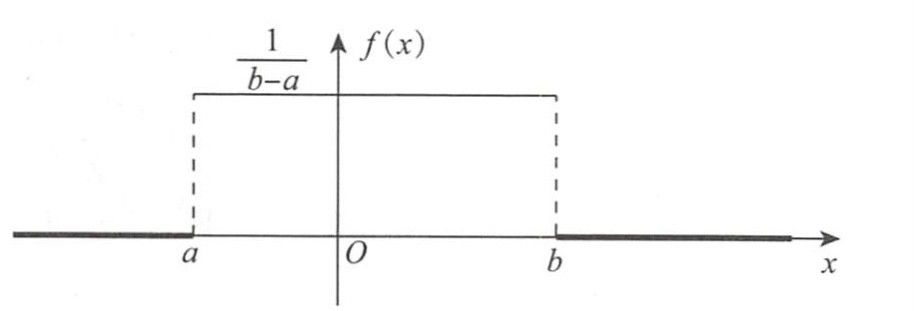
\includegraphics[width=0.45\textwidth]{"figure/Note/均匀分布1.jpg"}}
		\subfigure[分布函数]{
			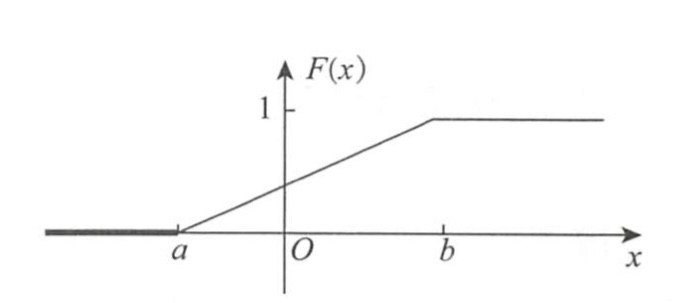
\includegraphics[width=0.45\textwidth]{"figure/Note/均匀分布2.jpg"}}
	\end{figure}
	\mathcolorbox{yellow}{(2). \text{指数分布}}
	
	$X\sim E(\lambda)$$X$的概率密度函数$f(x)$和分布函数$F(x)$: 
	$$f(x)=\left\lbrace 
	\begin{array}{l}
		\lambda e^{-\lambda x},\ x>0\\
		0,\ x\leq 0
	\end{array}
	\right. ,\ F(x)=\left\lbrace 
	\begin{array}{l}
		1-e^{-\lambda x},\ x\geq 0\\
		0,\ x<0
	\end{array}
	\right. (\lambda>0)$$
	\begin{figure}[H]
		\centering  %图片全局居中
		\subfigure[概率密度]{
			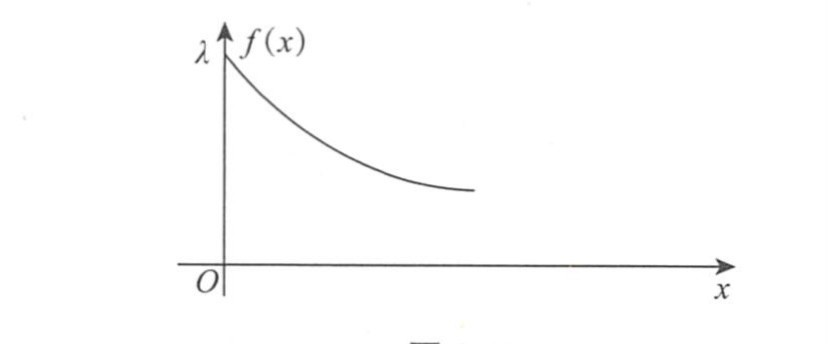
\includegraphics[width=0.45\textwidth]{"figure/Note/指数分布1.jpg"}}
		\subfigure[分布函数]{
			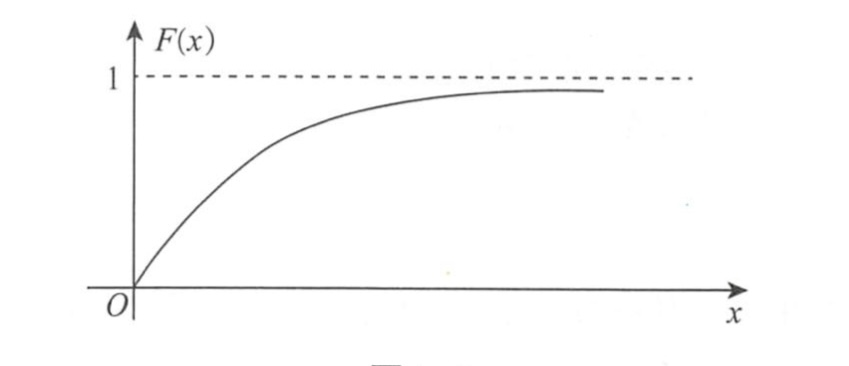
\includegraphics[width=0.45\textwidth]{"figure/Note/指数分布2.jpg"}}
	\end{figure}
	\mathcolorbox{yellow}{(3). \text{正态分布}}
	
	$X\sim N(\mu,\sigma^2)$,$X$的概率密度$f(x)$: 
	$$f(x)=\dfrac{1}{\sqrt{2\pi\sigma}}e^{-\frac{1}{2}(\frac{x-\mu}{\sigma})^2},(-\infty<x<+\infty) $$
	特别的,当$\mu=0,\sigma=1$时,$X\sim f(x)$是标准正态分布: 
	$$f(x)=\dfrac{1}{\sqrt{2\pi}}e^{-\frac{1}{2}x^2},(-\infty<x<+\infty)$$
	
	关于正态分布,我们有: 
	$$F(x)=P(X\leq x)=\varPhi(\dfrac{x-\mu}{\sigma})$$
	$$P(a\leq x\leq b)=\varPhi(\dfrac{b-u}{\sigma})-\varPhi(\dfrac{a-\mu}{\sigma})$$
	$$F(\mu-x)+F(\mu+x)=1,\ aX+b\sim N(a\mu+b,a^2\sigma^2)$$
	\begin{figure}[H]
		\centering  %图片全局居中
		\subfigure[概率密度]{
			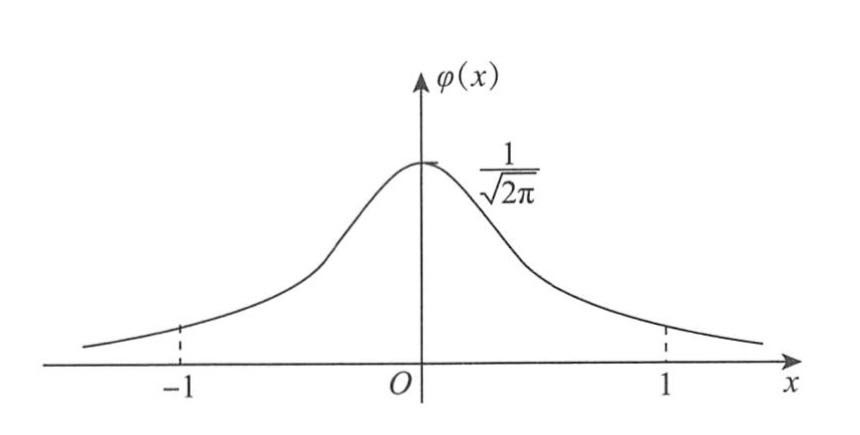
\includegraphics[width=0.45\textwidth]{"figure/Note/正态分布2.jpg"}}
		\subfigure[分布函数]{
			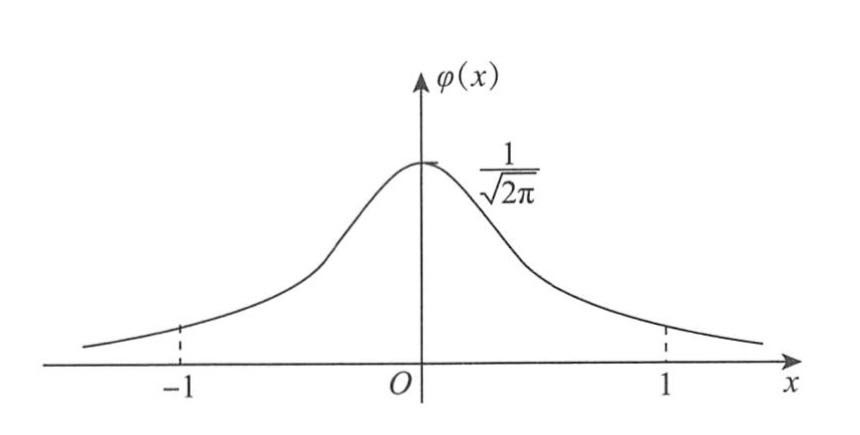
\includegraphics[width=0.45\textwidth]{"figure/Note/正态分布2.jpg"}}
	\end{figure}
\end{definition}
\section{一维随机变量函数的分布}
\begin{definition}
	设$X$是随机变量,函数$y=g(x)$,以随机变量$X$作为自变量的函数$Y=g(X)$也是随机变量,称为随机变量函数.
	
	我们一般有离散型$\rightarrow$离散型和连续型$\rightarrow$离散型两种随机变量函数.
\end{definition}
\chapterimage{chap23.jpg}
\chapter{多维随机变量及其分布}
\section{基本概念}
\begin{definition}[$n$维随机变量]
	如果$X_{1},X_{2},\cdots,X_{n}$是定义在同一个样本空间$\Omega$上的$n$个随机变量,我们称$(X_{1},X_{2},\cdots,X_{n})$为$n$维随机向量.
	
	对于任意的$n$个实数$x_{1},x_{2},\cdots,x_{n}$,我们把$n$元函数
	$$F(x_{1},x_{2},\cdots,x_{n})=P\{X_{1}\leq x_{1},X_{2}\leq x_{2},\cdots,X_{n}\leq x_{n}\}$$
	
	称为$n$维随机向量$(X_{1},X_{2},\cdots,X_{n})$的\textbf{联合分布函数}
	
	特别的,当$n=2$时,记$(X,Y)$为\textbf{二维随机变量}或者\textbf{二维随机向量},我们称$F(x,y)=P\{X\leq x,Y\leq y\}$为二维随机变量$(X,Y)$的联合分布函数,记作: 
	$$(X,Y)\sim F(x,y)\Leftrightarrow F(x,y)=P\{X\leq x,Y\leq y\}$$
	
	随机变量$X$与$Y$的分布函数$F_{X}(x)$和$F_{Y}(y)$分别称为随机变量关于$(X,Y)$关于$X$和$Y$的边缘分布函数.
	$$F_{X}(x)=P\{X\leq x\}=P\{X\leq x,Y< +\infty\}=F(x,+\infty)$$
	$$F_{Y}(y)=P\{Y\leq y\}=P\{X<+\infty,Y\leq y\}=F(+\infty,y)$$
	\begin{anymark}[注]
		\mathcolorbox{yellow}{\text{二维随机变量联合分布性质}}
		
		(1).单调性(单调不减)
		$$\forall x,\ \text{当}y_{1}<y_{2}\text{时},F(x,y_{1})\leq F(x,y_{2})$$
		$$\forall y,\ \text{当}x_{1}<x_{2}\text{时},F(x_{1},y)\leq F(x_{1},y)$$
		
		(2). 右连续性
		$$\lim\limits_{x\rightarrow x_{0}^{+}}F(x,y)=F(x_{0}+0,y)=F(x_{0},y)$$
		$$\lim\limits_{y\rightarrow y_{0}^{+}}F(x,y)=F(x,y_{0}+0)=F(x,y_{0})$$
		
		(3).有界性
		$$F(-\infty,y)=F(x,-\infty)=F(-\infty,-\infty)=0,\ F(+\infty,+\infty)=1$$
		
		(4).非负性
		$\forall x_{1}<x_{2},y_{1}<y_{2},\text{我们有}$: 
		$$F(x_{1}<x\leq x_{2},y_{1}<y\leq y_{2})=F(x_{2},y_{2})-F(x_{2},y_{1})-F(x_{1},y_{2})+F(x_{1},y_{1})\geq 0$$
	\end{anymark}
	
\end{definition}

\section{二维离散型随机变量}
\begin{table}[ht]
	\centering
	\caption{离散型二维随机变量概率分布}
	\label{table: 离散型二维随机变量概率分布}
	\begin{tblr}{
			hline{1,Z} = {2pt},
			hline{2,Y} = {1pt},
			vline{2,Y} = {1pt},
			cells = {$},
			cell{1}{1} = {mode = text}
	}
		\diagbox{$X$}{$Y$}                     & y_{1}  & \cdots & y_{j}  & \cdots & P\left\lbrace X=x_{i}\right\rbrace \\
		x_{1}                                  & p_{11} & \cdots & p_{1j} & \cdots & p_{1*}                             \\
		\vdots                                 & \vdots &        & \vdots &        & \vdots                             \\
		x_{i}                                  & p_{i1} & \cdots & p_{ij} & \cdots & p_{i*}                             \\
		\vdots                                 & \vdots &        & \vdots &        & \vdots                             \\
		P\left\lbrace Y=y_{j}\right\rbrace     & p_{*1} & \cdots & p_{*j} & \cdots & 1                                  \\
	\end{tblr}
\end{table}
\begin{definition}[二维离散型随机变量]
	\mathcolorbox{yellow}{\text{1.概率分布}}
	
	二维随机变量$(X,Y)$只能取有限对值或可列对值$(x_{1},y_{1}),(x_{2},y_{2}),\cdots,(x_{n},y_{n}),\cdots$,则称$(X,Y)$为离散型随机变量,$(X,Y)$满足概率分布: 
	$$p_{ij}=P\{X=x_{i},Y=y_{j}\},i,j=1,2,\cdots$$
	
	上面的式子称为$(X,Y)$的联合分布律,记作$(X,Y)\sim p_{ij}$,如 $\mathbf{table: }$ \ref{table: 离散型二维随机变量概率分布}所示
	
	$\text{数列}\{p_{ij}\},i,j=1,2,\cdots\text{是某一二维随机变量的概率分布的充要条件: }$
	$$ p_{ij}\geq 0,\ \sum\limits_{i=1}^{\infty}\sum\limits_{j=1}^{\infty}p_{ij}=1$$
	
	\mathcolorbox{yellow}{\text{2. 联合分布函数、边缘分布、条件分布}}
	
	(1). 联合分布函数
	$$F(x,y)=P\{X\leq x,Y\leq y\}=\sum\limits_{i=1}^{\infty}\sum\limits_{j=1}^{\infty}p_{ij}$$
	
	(2). 边缘分布
	
	$X$的边缘分布: 
	$$p_{i*}=P\{X=x_{i}\}=\sum\limits_{j=1}^{\infty}P\{X=x_{i},Y=y_{j}\}=\sum\limits_{j=1}^{\infty}p_{ij},(i=1,2,\cdots)$$
	$Y$的边缘分布: 
	$$p_{*j}=P\{Y=y_{j}\}=\sum\limits_{i=1}^{\infty}P\{X=x_{i},Y=y_{j}\}=\sum\limits_{i=1}^{\infty}p_{ij},(j=1,2,\cdots)$$
	
	(3). 条件分布
	
	$X$在$Y=y_{j}$下的条件分布: 
	$$P\{X=x_{i}|Y=y_{j}\}=\dfrac{P\{X=x_{i},Y=y_{j}\}}{P\{Y=y_{j}\}}=\dfrac{p_{ij}}{p_{*j}},i=1,2,\cdots$$
	$Y$在$X=x_{i}$下的条件分布: 
	$$P\{Y=y_{j}|X=x_{i}\}=\dfrac{P\{X=x_{i},Y=y_{j}\}}{P\{X=x_{i}\}}=\dfrac{p_{ij}}{p_{i*}},j=1,2,\cdots$$
\end{definition}
\section{二维连续型随机变量}
\begin{definition}[二维连续型随机变量]
	\mathcolorbox{yellow}{\text{1. 联合分布函数、概率密度}}
	$$F(x,y)=\int_{-\infty}^{x}\int_{-\infty}^{y}f(u,v)dudv,(x,y)\in\mathbb{R}^2$$
	
	$F(x,y)$是二维随机变量$(X,Y)$的概率分布函数,$f(x)$是二维随机变量$(X,Y)$的概率密度函数.
	
	$$f(x,y)\geq 0,\ \int_{-\infty}^{+\infty}\int_{-\infty}^{+\infty}f(x,y)dxdy$$
	\begin{anymark}[注]
		\begin{itemize}
			\item $f(x,y)$在点$(x_{0},y_{0})$处连续,我们有: $\dfrac{\partial^2 F(x,y)}{\partial x\partial y}|_{(x_{0},y_{0})}=f(x_{0},y_{0})$
			
			\item $F(x,y)$连续且可导,$\dfrac{\partial^2 F(x,y)}{\partial x\partial y}=f(x,y)$
		\end{itemize}
	\end{anymark}
	\mathcolorbox{yellow}{\text{2. 边缘分布函数、边缘概率密度}}
	
	$(X,Y)\sim f(x,y)$,$X$的边缘分布函数和边缘概率密度: 
	
	\mathcolorbox{orange}{\text{边缘分布函数}}
	\begin{flalign*}
		 F_{X}(x)=F(x,+\infty)=\int_{-\infty}^{x}\left[ \int_{-\infty}^{+\infty}f(u,v)dv\right] du
	\end{flalign*}
	
	\mathcolorbox{orange}{\text{边缘概率密度}}
	\begin{flalign*}
		f_{X}(x)=\int_{-\infty}^{+\infty}f(x,y)dy
	\end{flalign*}
	
	$(X,Y)\sim f(x,y)$,$Y$的边缘分布函数和边缘密度函数: 
	
	\mathcolorbox{orange}{\text{边缘分布函数}}
	\begin{flalign*}
		 F_{Y}(y)=F(+\infty,y)=\int_{-\infty}^{y}\left[ \int_{-\infty}^{+\infty}f(u,v)du\right] dv
	\end{flalign*}
	
	\mathcolorbox{orange}{\text{边缘概率密度}}
	\begin{flalign*}
		f_{Y}(y)=\int_{-\infty}^{+\infty}f(x,y)dx
	\end{flalign*}
	
	\mathcolorbox{orange}{\text{3. 条件分布函数、条件概率密度}}
	
	$(X,Y)\sim f(x,y)$,$X$在$Y=y$条件下的条件分布函数和条件概率密度: 
	
	\mathcolorbox{orange}{\text{条件概率密度}}
	\begin{flalign*}
	 f_{X|Y}(x|y)=\dfrac{f(x,y)}{f_{Y}(y)},(f_{Y}(y)>0)
	\end{flalign*}
	
	\mathcolorbox{orange}{\text{条件分布函数}}
	\begin{flalign*}
	 F_{X|Y}(x|y)=\int_{-\infty}^{x}f_{X|Y}(x|y)dx=\int_{-\infty}^{x}\dfrac{f(x,y)}{f_{Y}(y)}dx
	\end{flalign*}

	$(X,Y)\sim f(x,y)$,$Y$在$X=x$条件下的条件分布函数和条件概率密度: 
	
	\mathcolorbox{orange}{\text{条件概率密度}}
	\begin{flalign*}
	 f_{Y|X}(y|x)=\dfrac{f(x,y)}{f_{X}(x)},(f_{X}(x)>0)
	\end{flalign*}
	
	\mathcolorbox{orange}{\text{条件分布函数}}
	\begin{flalign*}
	 F_{Y|X}(y|x)=\int_{-\infty}^{y}f_{Y|X}(y|x)dy=\int_{-\infty}^{y}\dfrac{f(x,y)}{f_{X}(x)}dy
	\end{flalign*}
	
\end{definition}
\begin{definition}[常见二维分布]
	\mathcolorbox{skyblue}{\text{(1).二维均匀分布}}
	
	$(X,Y)$在有界区域$D$服从均匀分布,$(X,Y)$的概率密度为: 
	$$f(x,y)=\left\lbrace 
	\begin{array}{l}
		\dfrac{1}{S_{D}},\ (x,y)\in D\\
		0,\text{其他}
	\end{array}
	\right. S_{D}\text{是区域的面积}$$
	
	\mathcolorbox{skyblue}{\text{(2).二维正态分布}}
	
	$(X,Y)$概率密度为: 
	$$f(x,y)=\dfrac{1}{2\pi\sigma_{1}\sigma_{2}\sqrt{1-\rho^2}}exp\left\lbrace -\dfrac{1}{2(1-\rho^2)}\left[ \left( \dfrac{x-\mu_{1}}{\sigma_{1}}\right)^2-2\rho\left( \dfrac{x-\mu_{1}}{\sigma_{1}}\right)\left( \dfrac{x-\mu_{2}}{\sigma_{2}}\right) +\left( \dfrac{x-\mu_{2}}{\sigma_{2}}\right)^2\right] \right\rbrace $$
	
	其中$\mu_{1},\mu_{2}\in\mathbb{R},\ \sigma_{1},\sigma_{2}>0,-1<\rho<1$,我们称$(X,Y)$服从参数为$\mu_{1},\mu_{2},\sigma_{1},\sigma_{2},\rho$的二维正态分布,记作$(X,Y)\sim N(\mu_{1},\mu_{2};\sigma_{1}^2,\sigma_{2}^2;\rho)$
	
	\begin{anymark}[注]
		\begin{itemize}
			\item  $X\sim N(\mu_{1},\sigma_{1}^2)$,$Y\sim N(\mu_{2},\sigma_{2}^2)$,$\rho$是$X$与$Y$的相关系数
			$$\rho=\dfrac{Cov(X,Y)}{\sqrt{DX}\sqrt{DY}}=\dfrac{Cov(X,Y)}{\sigma_{1}\sigma_{2}}$$
			\item $X$和$Y$的条件分布都是正态分布
			\item $aX+bY(a\neq 0\text{或者}b\neq 0)$服从正态分布
			\item $X,Y$相互独立的充要条件为$X,Y$不相关$\Leftrightarrow \rho=0$
		\end{itemize}
	\end{anymark}
\end{definition}
\section{独立性}
\begin{definition}[独立性]
	1.概念
	
	设二维随机变量$(X,Y)$的联合分布$F(x,y)$,边缘分布分别为$F_{X}(x)$和$F_{Y}(y)$,如果对任意实数$(x,y)$,我们都有: 
	$$F(x,y)=F_{X}(x)F_{Y}(y)\Leftrightarrow X\text{和}Y\text{相互独立}$$
	
	\begin{itemize}
		\item 随机变量$X_{1},X_{2},\cdots,X_{n}$相互独立$\Leftrightarrow F(x_{1},x_{1},\cdots,x_{n})=F(x_{1})\dots F(x_{2})\cdots F(x_{n})$
		\item $X_{1},X_{2},\cdots,X_{n}$相互独立,则其中任意$k(2\leq k\leq n)$个随机变量也相互独立
		\item 两个多维随机变量$(X_{1},X_{2},\cdots,X_{n})$与$(Y_{1},Y_{2},\cdots,Y_{m})$相互独立,我们有: 
		$$F(x_{1},x_{2},\cdots,x_{n},y_{1},y_{2},\cdots,y_{m})=F_{1}(x_{1},x_{2},\cdots,x_{n})\dots F_{2}(y_{1},y_{2},\cdots,y_{m})$$
		\item $(X,Y)$为独立的二维随机变量,边缘分布和条件分布相等,边缘概率密度与条件概率密度相等.$(P\{Y=y_{j}\}>0,\ P\{X=x_{i}\}>0)$
		$$P\{X=x_{i}|Y=y_{j}\}=P\{X=x_{i}\},\ P\{Y=y_{j}|X=x_{i}\}=P\{Y=y_{j}\}$$
		$$f_{X|Y}(x|y)=\dfrac{f(x,y)}{f_{Y}(y)}=f_{X}(x)(f_{Y}(y)>0),\ f_{Y|X}(y|x)=\dfrac{f(x,y)}{f_{X}(x)}=f_{Y}(y)(f_{X}(x)>0)$$
	\end{itemize}
\end{definition}
\begin{definition}[连续型多维随机变量函数的分布]
	$(X,Y)\sim f(x,y)$
	
	\mathcolorbox{skyblue}{\text{(1).和的分布}}
	\begin{figure}[H]
		\centering  %图片全局居中
		\subfigure[$X+Y$]{
			\includegraphics[width=0.6\textwidth]{"figure/Note/和.jpg"}}
	\end{figure}
	$Z=X+Y$
	
	分布函数: 
	$$F_{Z}(z)=P\{X+Y\leq z\}=\iint\limits_{D_{z}:x+y\leq z}f(x,y)d\sigma=\left\lbrace 
	\begin{array}{l}
		\int_{-\infty}^{+\infty}dx\int_{-\infty}^{z-x}f(x,y)dy\\
		\int_{-\infty}^{+\infty}dy\int_{-\infty}^{z-y}f(x,y)dx
	\end{array}
	\right. $$
	
	概率密度: 
	$$f_{Z}(z)=F'_{Z}(z)=\left\lbrace 
	\begin{array}{l}
		\int_{-\infty}^{+\infty}f(z-y,y)dy\\
		\int_{-\infty}^{+\infty}f(x,z-x)dx
	\end{array}
	\right. $$
	
	\mathcolorbox{skyblue}{\text{(2).差的分布}}
	\begin{figure}[H]
		\centering  %图片全局居中
		\subfigure[$X-Y$]{
			\includegraphics[width=0.6\textwidth]{"figure/Note/差.jpg"}}
	\end{figure}
	$Z=X-Y$
	
	分布函数: 
	$$F_{Z}(z)=P\{X-Y\leq z\}=\iint\limits_{D_{z}:x-y\leq z}f(x,y)d\sigma=\left\lbrace 
	\begin{array}{l}
		\int_{-\infty}^{+\infty}dx\int_{x-z}^{+\infty}f(x,y)dy\\
		\int_{-\infty}^{+\infty}dy\int_{-\infty}^{y+z}f(x,y)dx
	\end{array}
	\right. $$
	
	概率密度: 
	$$f_{Z}(z)=F'_{Z}(z)=\left\lbrace 
	\begin{array}{l}
		\int_{-\infty}^{+\infty}f(z+y,y)dy\\
		\int_{-\infty}^{+\infty}f(x,x-z)dx
	\end{array}
	\right. $$
	
	\mathcolorbox{skyblue}{\text{(3).积的分布}}
	\begin{figure}[H]
		\centering  %图片全局居中
		\subfigure[$XY$]{
			\includegraphics[width=0.6\textwidth]{"figure/Note/积.jpg"}}
	\end{figure}
	$Z=XY$
	
	分布函数: 
	\begin{eqnarray*}
		F_{Z}(z)&=&P\{XY\leq z\}=\iint\limits_{D_{z}:xy\leq z}f(x,y)d\sigma\\
		&=&\left\lbrace 
		\begin{array}{l}
			\int_{-\infty}^{0}dy\int_{\frac{z}{y}}^{+\infty}f(x,y)dx+\int_{0}^{+\infty}dy\int_{-\infty}^{\frac{z}{y}}f(x,y)dx\\
			\int_{-\infty}^{0}dx\int_{\frac{z}{x}}^{+\infty}f(x,y)dy+\int_{0}^{+\infty}dx\int_{-\infty}^{\frac{z}{x}}f(x,y)dy
		\end{array}
		\right.
	\end{eqnarray*}
	
	概率密度: 
	$$f_{Z}(z)=F'_{Z}(z)=\left\lbrace 
	\begin{array}{l}
		\int_{-\infty}^{0}(-\frac{1}{y})f(\frac{z}{y},y)dy+\int_{0}^{+\infty}\frac{1}{y}f(\frac{z}{y},y)dy=\int_{-\infty}^{+\infty}\frac{1}{|y|}f(\frac{z}{y},y)dy\\
		\int_{-\infty}^{0}(-\frac{1}{x})f(x,\frac{z}{x})dx+\int_{0}^{+\infty}\frac{1}{x}f(x,\frac{z}{x})dx=\int_{-\infty}^{+\infty}\frac{1}{|x|}f(x,\frac{z}{x})dx
	\end{array}
	\right. $$
	
	\mathcolorbox{skyblue}{\text{(4).商的分布}}
	\begin{figure}[H]
		\centering  %图片全局居中
		\subfigure[$\dfrac{X}{Y}$]{
			\includegraphics[width=0.6\textwidth]{"figure/Note/商.jpg"}}
	\end{figure}
	$Z=\dfrac{X}{Y}$
	
	分布函数: 
	$$F_{Z}(z)=P\{\dfrac{X}{Y}\leq z\}=\iint\limits_{D_{z}:\frac{X}{Y}\leq z}f(x,y)d\sigma=\int_{-\infty}^{0}dy\int_{zy}^{+\infty}f(x,y)dx+\int_{0}^{+\infty}dy\int_{-\infty}^{zy}f(x,y)dx$$
	
	概率密度: 
	$$f_{Z}(z)=F'_{Z}(z)=\int_{-\infty}^{0}(-y)f(zy,y)dy+\int_{0}^{+\infty}yf(zy,y)dy=\int_{-\infty}^{+\infty}|y|f(zy,y)dy$$
	
	\mathcolorbox{skyblue}{\text{(5).}max\{X,Y\}}
	
	$Z=max\{X,Y\}$
	
	分布函数: 
	\begin{eqnarray*}
		F_{Z}(z)=P\{Z\leq max\{X,Y\}\}&=&P\{X\leq z\}\cup P\{Y\leq z\}\\
		&=&P\{X\leq z\}+P\{Y\leq z\}-P\{X\leq z,Y\leq z\}\\
		&=&F_{X}(z)+F_{Y}(z)-F(z,z)
	\end{eqnarray*}

	
	概率密度: 
	$$f_{Z}=F'_{Z}(z)=f(z,z)$$
	
	\mathcolorbox{skyblue}{\text{(6).}min\{X,Y\}}
	
	$Z=min\{X,Y\}$
	
	分布函数: 
	$$F_{Z}(z)=P\{Z\leq min\{X,Y\}\}=P\{X\leq z,Y\leq z\}=F(z,z)\Rightarrow F_{max}(z)=F(z,z)$$
	
	概率密度: 
	$$f_{Z}=F'_{Z}(z)=f_{X}(z)+f_{Y}(z)-f(z,z)$$
	\begin{anymark}[注]
		\begin{itemize}
			\item  $n$个相互独立的随机变量$X_{1},X_{2},\cdots,X_{n}$,$Z_{1}=max\{X_{1},X_{2},\cdots,X_{n}\},\ Z_{2}=min\{X_{1},X_{2},\cdots,X_{n}\}$,$Z_{1},Z_{2}$的分布函数: 
			$$F_{max}(z)=F_{X_{1}}(z)F_{X_{2}}(z)\cdots F_{X_{n}}(z)$$
			$$F_{min}(z)=1-[1-F_{Z_{1}}(z)][1-F_{Z_{2}}(z)]\cdots[1-F_{Z_{n}}(z)]              $$
			\item $X_{i}(i=1,2,\cdots,n)$独立同分布,我们有: 
			$$F_{max}(x)=[F(x)]^n,\ f_{max}(x)=n[F(x)]^{n-1}f(x)$$
			$$F_{min}(x)=1-[1-F(x)]^n,\ f_{min}(x)=nf(x)[1-F(x)]^{n-1}$$
		\end{itemize}
	\end{anymark}
\end{definition}
\begin{table}[ht]
	\centering
	\caption{常见分布可加性}
	\label{table: 常见分布可加性}
	\begin{tblr}{
		hlines,
		vline{2,3},
		cells = {c,$}
	}
		X                       & Y                       & X+Y                                         \\
		B(n,p)                  & B(m,p)                  & B(n+m,p)                                    \\
		P(\lambda_{1})          & P(\lambda_{2})          & P(\lambda_{1}+\lambda_{2})                  \\
		N(\mu_{1},\sigma_{1}^2) & N(\mu_{2},\sigma_{2}^2) & N(\mu_{1}+\mu_{2},\sigma_{1}^2+\sigma_{2}^2)\\
		\chi^2(n)               & \chi^2(m)               & \chi^2(n+m)                                 \\
	\end{tblr}
\end{table}
\chapterimage{chap24.jpg}
\chapter{随机变量的数字特征}
\section{一维随机变量的数字特征}
\begin{definition}[数学期望]
		1. $X$是离散型随机变量,$X$的分布列为$p_{i}=P\{X=x_{i}\}(i=1,2,\cdots,n)$,如果级数$\sum\limits_{i=1}^{+\infty}x_{i}p_{i}$绝对收敛,我们称随机变量$X$的数学期望存在,并将其记作$E(X)$.
	$$E(X)=\sum\limits_{i=1}^{+\infty}x_{i}p_{i}$$
	
	2. $X$是连续型随机变量,$X$的概率密度为$f(x)$,如果积分$\int_{-\infty}^{+\infty}xf(x)dx$绝对收敛,我们称随机变量$X$的数学期望存在,并将其记作$E(X)$.
	$$E(X)=\int_{-\infty}^{+\infty}xf(x)dx$$
	\begin{itemize}
		\item  $a_{i}\text{为常数,}E\left(\sum\limits_{i=1}^{n}a_{i}X_{i} \right)=\sum\limits_{i=1}^{n}a_{i}E(X_{i}) $
		\item $E(X\pm Y)=E(X)\pm E(Y),\ E(aX+bY)=aE(X)+bE(Y)$
		\item $X\text{与}Y\text{相互独立}\Rightarrow E(XY)=E(X)E(Y),E\left[g_{1}(X)\dots g_{2}(Y) \right]=E\left[g_{1}(X)\right]\dots E\left[g_{2}(Y) \right] $
		\item $X_{1},X_{2},\cdots,X_{n}$相互独立,我们有: 
		$$E\left( \prod\limits_{i=1}^{n}X_{i}\right)=\prod\limits_{i=1}^{n}E(X_{i}),\ E\left[\prod\limits_{i=1}^{n}g_{i}(X_{i}) \right]=\prod\limits_{i=1}^{n}E\left[g_{i}(X_{i}) \right]   $$
	\end{itemize}
\end{definition}
\begin{definition}[方差和标准差]
	设$X$是随机变量,如果$E[(X-EX)^2]$存在,我们将$E[(X-EX)^2]$记作$X$的方差$D(X)(DX)$: 
	$$D(X)=E[(X-EX)^2]=E(X^2)-[E(X)]^2$$
	
	我们将$\sqrt{D(X)}$称为随机变量的\textbf{标准差}或者\textbf{均方差},记作$\sigma(X)$.
	\begin{itemize}
		\item $DX\geq 0,\ E(X^2)=DX+(EX)^2$
		\item $D(c)=0,\ c\text{为常数}$
		\item $D(aX+b)=a^2D(X),\ D(X+b)=D(X)$ 
		\item $D(X\pm Y)=D(X)+D(Y)\pm 2Cov(X,Y)$
		\item $X^{*}=\dfrac{X-E(X)}{\sigma(X)}$是$X$的标准化随机变量,$E(X^{*})=0,D(X^{*})=1$
		\item $\text{如果}X\text{和}Y\text{相互独立,我们得到}$
		$$D(aX+bY)=a^2D(X)+b^2D(Y)$$
		\item $X_{1},X_{2},\cdots,X_{n}$是相互独立,我们有: 
		$$D\left( \sum\limits_{i=1}^{n}a_{i}X_{i}\right)=\sum\limits_{i=1}^{n}a_{i}^2D(X_{i})$$
		$$D\left( \sum\limits_{i=1}^{n}g_{i}(X_{i})\right)=\sum\limits_{i=1}^{n}D\left[ g_{i}(X_{i})\right]  $$
	\end{itemize}
\end{definition}
\begin{definition}[切比雪夫不等式]
	如果随机变量$X$的期望$E(X)$和方差$D(X)$都存在,对任意$\varepsilon>0$,我们都有: 
	$$\mathcolorbox{purplea}{P\{|X-E(X)|\geq \varepsilon\}\leq \dfrac{D(X)}{\varepsilon^2}\text{或者}P\{|X-E(X)|< \varepsilon\}\geq 1-\dfrac{D(X)}{\varepsilon^2}}$$
	\begin{anymark}[注]
		
	\end{anymark}
\end{definition}

\section{二维随机变量的数字特征}
\begin{definition}[数学期望]
设 $X,Y$为随机变量,$g(X,Y)$为$X,Y$的函数($g$是连续函数)

1. $(X,Y)$是离散型随机变量,联合分布为: 
$$p_{ij}=P\{X=x_{i},Y=y_{j}\}(i,j=1,2,\cdots)$$

级数$\sum\limits_{i}\sum\limits_{j}g(x_{i},y_{j})p_{ij}$绝对收敛,我们定义: 
$$E[g(X,Y)]=\sum\limits_{i}\sum\limits_{j}g(x_{i},y_{j})p_{ij}$$

2. $(X,Y)$是连续型随机变量,概率密度为$f(x,y)$,积分$\int_{-\infty}^{+\infty}\int_{-\infty}^{+\infty}f(x,y)dxdy$绝对收敛,我们定义: 
$$E[g(X,Y)]=\int_{-\infty}^{+\infty}\int_{-\infty}^{+\infty}f(x,y)dxdy$$
\end{definition}
\begin{definition}[协方差与相关系数]
如果随机变量$X$与$Y$的方差存在且$D(X)>0,D(Y)>0$,我们定义随机变量$X,Y$的协方差$Cov(X,Y)$: 

$$Cov(X,Y)=E[(X-E(X))(Y-E(Y))]=E(XY)-E(X)E(Y)$$

其中$E(XY)$: 
$$E(XY)=\left\lbrace 
\begin{array}{l}
\sum\limits_{i}\sum\limits_{j}x_{i}y_{i}p_{ij},\ (X,Y)\text{是离散型随机变量}\\
\int_{-\infty}^{+\infty}\int_{-\infty}^{+\infty}xyf(x,y)dxdy,\ (X,Y)\text{是连续型随机变量}
\end{array}
\right. $$
	
我们将$\rho_{XY}=\dfrac{Cov(X,Y)}{\sqrt{DX}\sqrt{DY}}$定义为随机变量$X,Y$的\textbf{相关系数}.
\begin{itemize}
	\item $\rho_{XY}=0\Rightarrow X,Y\text{不相关}$
	\item $\rho_{XY}\neq0\Rightarrow X,Y\text{相关}$
	\item $\text{对称性}\  Cov(X,Y)=Cov(Y,X),\ Cov(X,X)=D(X),\ \rho_{XX}=1$
	\item $\text{线性} \ Cov(aX+b,Y)=aCov(X,Y),\ Cov(X_{1}+X_{2},Y)=Cov(X_{1},Y)+Cov(X_{2},Y)$
\end{itemize}
\end{definition}

\begin{table}[ht]
	\centering
	\caption{常用分布表}
	\label{table: 常用分布表}
	\begin{tblr}{
		hlines = {1pt},
		hline{1,Z} = {2pt},
		vline{2-Y} = {1pt},
		cells = {c}
	}
		$\text{名称}$                                    & $\text{概率分布}$                                                                    & $\text{均值}$            & $\text{方差}$                      & $\text{参数范围}$                       \\
		$\text{两点分布}$                                & {$P(X=k)=p^kq^{1-k}$\\ $(k=0,1)$}                                                   & $p$                      & $pq$                              & {$0<p<1$\\ $q=1-p$}                     \\
		{$\text{二项分布}$\\ $B(n,p)$}                   & {$P(X=k)=C_{n}^{k}p^xq^{n-k}$ \\ $(x=0,1,\cdots,n)$}                                & $np$                     & $npq$                             & {$0<p<1$ \\ $q=1-p$\\ $n\in N$}         \\
		{$\text{泊松分布}$\\ $P(\lambda$)}               & {$P(X=k)=\dfrac{\lambda^k}{k!}e^{-\lambda}$ \\ $(k=0,1,2,\cdots)$}                  & $\lambda$                & $\lambda$                         & $\lambda>0$                             \\
		{$\text{超几何分布}$\\ $H(n,N,M)$}               & {$P(X=k)=\dfrac{C_{N-M}^{n-k}C_{M}^{k}}{C_{N}^{n}}$\\ $(k=0,1,\cdots\,min\{M,n\})$} & $\dfrac{nM}{N}$          & $\dfrac{n(N-n)(N-M)M}{N^2(N-1)}$  & {$n,N,M\in N$\\ $n\leq N,M\leq N$}      \\
		{$\text{几何分布}$\\ $G(p)$}                     & {$P(X=k)=(1-p)^{k-1}p$\\ $(k=0,1,\cdots)$}                                          & $\dfrac{1}{p}$           & $\dfrac{1-p}{p^2}$                & {$0<p<1$\\ $q=1-p$}                     \\
		{$\text{均匀分布}$\\ $U(a,b)$}                   & $p(x)=\frac{1}{b-a}(a\leq x\leq b)$                                                 & $\dfrac{a+b}{2}$         & $\dfrac{(b-a)^3}{12}$             & {$0<p<1$\\ $q=1-p$\\ $r\in \mathbb{R}$} \\
		{$\text{指数分布}$\\ $E(\lambda)$}               & $p(x)=\lambda e^{-\lambda x}(x>0)$                                                  & $\dfrac{1}{\lambda}$     & $\dfrac{1}{\lambda^2}$            & $\lambda>0$                             \\
		{$\text{正态分布}$\\ $N(\mu,\sigma^2)$}          & $p(x)=\dfrac{1}{\sqrt{2\pi\sigma}}e^{-\dfrac{(x-\mu)^2}{2\sigma^2}}$                & $\mu$                    & $\sigma^2$                        & $\sigma>0$                              \\
		{$\Gamma\text{分布}$ \\ $\Gamma(\alpha,\beta)$} & $p(x)=\dfrac{\beta^{\alpha}}{\Gamma(\alpha)}x^{\alpha-1}e^{-\beta x}(x>0)$           & $\dfrac{\alpha}{\beta}$ & $\dfrac{\alpha}{\beta^2}$          & {$\alpha>0$\\ $\beta>0$}                \\
	\end{tblr}
\end{table}
\chapterimage{chap25.jpg}
\chapter{大数定理和中心极限定理}
\section{依概率收敛}
\begin{definition}[依概率收敛]
	设随机变量$X$与随机变量序列$\{X_{n}\}(n=1,2,3,\cdots)$,如果对于任意$\varepsilon>0$,我们有: 
	$$\lim\limits_{n\Rightarrow \infty}P\{|X_{n}-X|\geq \varepsilon\}=0\text{或者}\lim\limits_{n\Rightarrow \infty}P\{|X_{n}-X|<\varepsilon\}=1$$
	
	我们称随机变量序列$\{X_{n}\}$\textbf{依概率收敛于随机变量}$X$,记作: 
	$$\lim\limits_{n\Rightarrow \infty}X_{n}=X(P)\text{或者}X_{n}\stackrel{P}{\longrightarrow}X(n\Rightarrow \infty)$$
\end{definition}
\section{大数定理}
\begin{theorem}[切比雪夫大数定理]
	假设$\{X_{n}\}(n=1,2,\cdots)$是相互独立的随机变量序列,如果方差$D(X_{i})$存在且一致有上界,即存在常数$C$,$\forall i\geq 1, s.t. D(X_{i})\leq C$,$\{X_{n}\}$服从大数定理.
	$$\dfrac{1}{n}\sum\limits_{i=1}^{n}X_{i}\stackrel{P}{\longrightarrow}\dfrac{1}{n}\sum\limits_{i=1}^{n}E(X_{i})$$
\end{theorem}
\begin{theorem}[伯努利大数定理]
	假设$\mu_{n}$是$n$重伯努利试验中事件$A$发生的次数,在每次试验中事件$A$发生的概率为$p(0<p<1)$,则$\dfrac{\mu_{n}}{n}\stackrel{P}{\longrightarrow}p$.
	$$\forall \varepsilon>0,\lim\limits_{n\Rightarrow \infty}P\{|\dfrac{\mu_{n}}{n}-p|<\varepsilon\}=1$$
\end{theorem}
\begin{theorem}[辛钦大数定理]
	假设$\{X_{n}\}$是独立同分布的随机变量序列,如果$E(X_{i})=\mu,(i=1,2,\cdots)$存在,则$\dfrac{1}{n}\sum\limits_{i=1}^{n}X_{i}\stackrel{P}{\longrightarrow}\mu$.
	$$\forall \varepsilon>0,\lim\limits_{n\Rightarrow \infty}P\{|\dfrac{1}{n}\sum\limits_{i=1}^{n}X_{i}-\mu|<\varepsilon\}=1$$
\end{theorem}
\section{中心极限定理}
\begin{theorem}[列维-林德伯格定理]
	假设$\{X_{n}\}$是独立同分布的随机变量序列,如果$E(X_{i})=\mu,D(X_{i})=\sigma^2>0,(i=1,2,\cdots)$
	存在,$\forall x\in \mathbb{R}$,我们有: 
	$$\lim\limits_{n\Rightarrow \infty}P\{\dfrac{\sum\limits_{i=1}^{n}X_{i}-n\mu}{\sqrt{n\sigma}}<x\}=\dfrac{1}{\sqrt{2\pi}}\int_{-\infty}^{x}e^{-\frac{t^2}{2}}dt=\varPhi(x)$$
\end{theorem}
\begin{anymark}[注]
	\begin{itemize}
		\item $\text{定理满足}X_{n}\text{独立同分布、方差和期望存在}$
		\item $\sum\limits_{i=1}^{n}X_{i}\sim N(n\mu,n\sigma^2)$
		\item $P\{a<\sum\limits_{i=1}^{n}X_{i}<b\}\approx\varPhi(\dfrac{b-n\mu}{\sqrt{n}\sigma})-\varPhi(\dfrac{a-n\mu}{\sqrt{n}\sigma})$
	\end{itemize}
\end{anymark}
\begin{theorem}[棣莫弗-拉普拉斯定理]
	假设随机变量$Y_{n}\sim B(n,p),(0<p<1,n\geq 1)$,$\forall x\in \mathbb{R}$,我们有: 
	$$\lim\limits_{n\Rightarrow \infty}P\{\dfrac{Y_{n}-np}{\sqrt{np(1-p)}}<x\}=\dfrac{1}{\sqrt{2\pi}}\int_{-\infty}^{x}e^{-\frac{t^2}{2}}dt=\varPhi(x)$$
\end{theorem}
这一部分的内容我推荐一个$B$站视频观看.
\begin{itemize}
	\item \href{https://www.bilibili.com/video/BV1gh4y1W7ag/?spm_id_from=333.999.list.card_archive.click}{中心极限定理}
	\item \href{https://www.bilibili.com/video/BV1wu411W7uU/?spm_id_from=333.999.list.card_archive.click}{正态分布}
\end{itemize}
\chapterimage{chap26.jpg}
\chapter{数理统计}
\section{总体和样本}
\begin{definition}[统计概念和统计量]
	1. \textbf{总体}: 研究对象的全体称为总体
	
	2. \textbf{样本}: $n$个相互独立且与总体具有相同概率分布的随机变量$X_{1},X_{2},\cdots,X_{n}$所组成的整体$(X_{1},X_{2},\cdots,X_{n})$称为来自总体$X$,容量为$n$的一个\textbf{简单随机样本},一次抽样结果的具体的$n$个数值$(x_{1},x_{2},\cdots,x_{n})$称为样本$(X_{1},X_{2},\cdots,X_{n})$的一个观测值.
	
	3. \textbf{样本分布}
	
	假设总体的分布函数$F(x)$,概率密度函数$f(x)$,样本$(X_{1},X_{2},\cdots,X_{n})$的分布函数和概率密度: 
	$$\text{离散型: }P\{X_{1}=x_{1},X_{2}=x_{2},\cdots,X_{n}=x_{n}\}=\prod\limits_{i=1}^{n}P\{X_{i}=x_{i}\}$$
	$$\text{连续型分布函数: }F(x_{1},x_{2},\cdots,x_{n})=\prod\limits_{i=1}^{n}F(x_{i})$$
	$$\text{连续型概率密度: }f(x_{1},x_{2},\cdots,x_{n})=\prod\limits_{i=1}^{n}f(x_{i})$$
\end{definition}
\section{统计量及其分布}
\begin{definition}
	设$X_{1},X_{2},\cdots,X_{n}$是来自总体$X$的一个样本,$g(x_{1},x_{2},\cdots,x_{n})$是$n$元函数,如果函数$g$中不含任何参数,我们称$g(X_{1},X_{2},\cdots,X_{n})$是样本$X_{1},X_{2},\cdots,X_{n}$的一个\textbf{统计量}.
	
	1. \textbf{常用统计量}
	
	(1).数字特征
	\begin{itemize}
		\item \textbf{样本均值(一阶原点矩)}\ $\overline{X}=\dfrac{1}{n}\sum\limits_{i=1}^{n}X_{i}$
		\item \textbf{样本方差(二阶中心矩)}\ $S^2=\dfrac{1}{n-1}\sum\limits_{i=1}^{n}(X_{1}-\overline{X})^2$
		\item \textbf{样本}k\text{阶原点矩}\ $A_{k}=\dfrac{1}{n}\sum\limits_{i=1}^{n}X_{i}^{k},(k=1,2,\cdots)$
		\item \textbf{样本}k\text{阶中心矩}\ $B_{k}=\dfrac{1}{n}\sum\limits_{i=1}^{n}(X_{i}-\overline{X})^{k},(k=2,\cdots)$
	\end{itemize}
	
	(2). 顺序统计量
	
	将样本$X_{1},X_{2},\cdots,X_{n}$的$n$个观测值从小到大顺序排序得到: 
	$$X_{(1)}\leq X_{(2)}\leq \cdots\leq X_{(n)}\leq$$
	
	随机变量$X_{(k)}$称作第$k$顺序统计量,$X_{(1)}$为最小顺序统计量,$X_{(n)}$为最大顺序统计量.
	\begin{anymark}[注]
		假设总体期望$E(X)=\mu$,总体方差为$D(X)=\sigma^2$,$X_{1},X_{2},\cdots,X_{n}$是取自总体的一个样本,$\overline{X},S^2$分别为样本的均值和方差,我们有: 
		
		1.$E(X_{i})=\mu$
		
		2.$D(X_{i})=\sigma^2$
		
		3.$E(\overline{X})=E(\dfrac{X_{1}+X_{2}+\cdots+X_{n}}{n})=E(X)=\mu$
		
		4.$E(S^2)=D(X)=\sigma^2$
		
		5.$D(\overline{X})=\dfrac{1}{n}D(X)=\dfrac{\sigma^2}{n}$
	\end{anymark}
\end{definition}
\begin{definition}[三大分布]
	1. $\chi^2$分布
	
	随机变量$X_{1},X_{2},\cdots,X_{n}$相互独立,且都服从标准正态分布,则随机变量$X=\sum\limits_{i=1}^{n}X_{i}^2$服从自由度为$n$的卡方分布$\chi^2(n)$,记作$X\sim \chi^2(n)$.
	
	$\alpha$分位点: $\text{对于给定的}\alpha(0<\alpha<1),\text{满足}$
	$$P\{\chi^2>\chi_{\alpha}^2(n)\}=\int_{\chi_{\alpha}^2(n)}^{+\infty}f(x)dx$$
	的$\chi_{\alpha}^2(n)$为$\chi^2(n)$分布上的$\alpha$分位点.
	\begin{itemize}
		\item $X_{1}\sim \chi^2(n_{1}),\ X_{2}\sim \chi^2(n_{2})$,$X_{1},X_{2}$相互独立,我们有: $X_{1}+X_{2}\sim \chi^2(n_{1}+n_{2})$
		\item $X\sim \chi^2(n)\Rightarrow E(X)=n,D(X)=2n$
	\end{itemize}
	2. $t$分布
	
	设随机变量$X\sim N(0,1)$,$Y\sim \chi^2(n)$,$X,Y$相互独立,记随机变量$t=\dfrac{X}{\sqrt{Y/n}}$服从自由度为$n$的$t$分布,记作$t\sim t(n)$
	
	\begin{itemize}
		\item $t_{1-\alpha}(n)=-t_{\alpha}(n)$
		\item $t$分布概率密度关于$x$轴对称
	\end{itemize}
	
	3. $F$分布
	
	设随机变量$X\sim \chi^2(n_{1}),Y\sim \chi^2(n_{2})$,且$X,Y$相互独立,则$F=\dfrac{X/n_{1}}{Y/n_{2}}$服从自由度为$(n_{1},n_{2})$的$F$分布,记作$F\sim F(n_{1},n_{2})$.
	
	\begin{itemize}
		\item $F\sim F(n_{1},n_{2})\Rightarrow \dfrac{1}{F}\sim F(n_{2},n_{1})$
		\item $F_{1-\alpha}(n_{1},n_{2})=\dfrac{1}{F_{\alpha}(n_{2},n_{1})}$
	\end{itemize}
\end{definition}
\begin{anymark}[注]
	正态总体条件下常见结论: 
	
	设$X_{1},X_{2},\cdots,X_{n}$是来自正态总体$N(\mu,\sigma^2)$的一个样本,$\overline{X},S^2$分别是样本的均值和方差.
	
	1. $\overline{X}\sim N(\mu,\dfrac{\sigma^2}{n})\Rightarrow \dfrac{\overline{X}-\mu}{\frac{\sigma}{\sqrt{n}}}=\dfrac{\sqrt{n}(\overline{X}-\mu)}{\sigma}\sim N(0,1)$
	
	2. $\dfrac{1}{\sigma^2}\sum\limits_{i=1}^{n}(X_{i}-\mu)^2\sim \chi^2(n)$
	
	3. $\dfrac{(n-1)S^2}{\sigma^2}=\sum\limits_{i=1}^{n}(\dfrac{X_{i}-\overline{X}}{\sigma})^2\sim \chi^2(n)$
	
	4. $\overline{X}$和$S^2$相互独立,$\dfrac{\sqrt{n}(\overline{X}-\mu)}{S}\sim t(n-1)$
	
	5. $\sigma\text{未知时}$: $\dfrac{n(\overline{X}-\mu)^2}{S^2}\sim F(1,n-1)$
\end{anymark}
\section{参数的点估计}
\begin{definition}[矩估计和最大似然估计]
	1. 概念
	
	设总体$X$的分布函数$F(x,\theta)$,其中$\theta$是一个未知参数,$X_{1},X_{2},\cdots,X_{n}$是来自总体的一个样本,由样本构造一个适当的统计量$\hat{\theta}(X_{1},X_{2},\cdots,X_{n})$作为参数$\theta$的估计,称统计量为参数的估计量,$\theta=\hat{\theta}(X_{1},X_{2},\cdots,X_{n})$.
	
	2. 矩估计法
	
	设总体分布中有$k$个未知的参数$\theta_{1},\theta_{2},\cdots,\theta_{k}$,来自总体$X$的一组样本$X_{1},X_{2},\cdots,X_{n}$,如果$X$的原点矩$E(X^{l})(l=1,2,\cdots,k)$存在,我们令样本的原点矩=总体原点矩: 
	$$\dfrac{1}{n}\sum\limits_{i=1}^{n}X_{i}^{l}=E(X^{l})=\left\lbrace 
	\begin{array}{l}
		\int_{-\infty}^{+\infty}x^{l}f(x;\theta_{1},\theta_{2},\cdots,\theta_{k})dx\\
		\sum\limits_{i=1}^{n}x_{i}^{l}P\{X=x_{i};\theta_{1},\theta_{2},\cdots,\theta_{k}\}
	\end{array}
	\right. $$
	
	3. 最大似然估计法
	对未知参数$\theta$进行估计,在该参数可能的取值范围$I$中选取,使用使样本观测值$x_{1},x_{2},\cdots,x_{n}$最大的参数$\hat{\theta}$作为参数$\theta$的估计值.
	
	(1).总体$X$是离散型分布,分布函数的参数为$\theta_{1},\theta_{2},\cdots,\theta_{k}$,样本$X_{1},X_{2},\cdots,X_{n}$出现取值$x_{1},x_{2},\cdots,x_{n}$的概率为: 
	$$P\{X_{1}=x_{1},X_{2}=x_{2},\cdots,X_{n}=x_{n}\}=\prod\limits_{i=1}^{n}P(X_{i}=x_{i})=\prod\limits_{i=1}^{n}p(x_{i};\theta)$$
	
	我们得到似然函数: 
	$$L(\theta)=L(x_{1},x_{2},\cdots,x_{n},\theta)$$
	
	$$\exists \hat{\theta}\in I,\ s.t. L(x_{1},x_{2},\cdots,x_{n},\hat{\theta})=max_{\theta\in I}L(x_{1},x_{2},\cdots,x_{n},\theta)$$
	
	(2).总体$X$是连续型分布,概率密度为$f(x;\theta),\theta\in I$,样本$X_{1},X_{2},\cdots,X_{n}$出现取值$x_{1},x_{2},\cdots,x_{n}$的概率为: 
	$$L(\theta)=L(x_{1},x_{2},\cdots,x_{n},\theta)=\prod\limits_{i=1}^{n}f(x_{i},\theta)$$
	
	$$\exists \hat{\theta}\in I,\ s.t. L(x_{1},x_{2},\cdots,x_{n},\hat{\theta})=max_{\theta\in I}L(x_{1},x_{2},\cdots,x_{n},\theta)$$
	
	我们得到了参数的最大似然估计$\hat{\theta}=\hat{\theta}(x_{1},x_{2},\cdots,x_{n})$
	\begin{anymark}[估计量的评判标准]
		1. 无偏性
		
		2. 有效性(最小方差性)
		
		3. 一致性(相和性)
	\end{anymark}
\end{definition}
\section{参数的区间估计}
\begin{definition}[概念]
	设$\theta$是总体$X$的一个未知参数,对于给定的$\alpha(0<\alpha<1)$,如果由样本$X_{1},X_{2},\cdots,X_{n}$确定的两个统计量$\hat{\theta_{1}}=\hat{\theta_{1}}(X_{1},X_{2},\cdots,X_{n})$和$\hat{\theta_{2}}=\hat{\theta_{2}}(X_{1},X_{2},\cdots,X_{n})$满足: 
	$$P\{\hat{\theta_{1}}(X_{1},X_{2},\cdots,X_{n})<\theta<\hat{\theta_{2}}(X_{1},X_{2},\cdots,X_{n})\}=1-\alpha$$
	
	则称随机区间$(\hat{\theta_{1}},\hat{\theta_{2}})$是$\theta$的置信度为$1-\alpha$的\textbf{置信区间},$\hat{\theta_{1}}$和$\hat{\theta_{2}}$分别称为\textbf{置信上限}和\textbf{置信下限},$1-\alpha$为置信水平,$\alpha$为显著性水平.
\end{definition}
\begin{table}[h]
	\centering
	\caption{正态总体均值的置信区间}
	\label{table: 正态总体均值的置信区间}
	\begin{tblr}{
		hline{1,Z} = {2pt},
		hline{2,Y} = {1pt},
		vline{2-Y} = {1pt},
		cells = {c,$}
	}
		\text{待估参数} & \text{其他参数}     & \text{枢轴量分布}                                        & \text{置信区间}                                                                                                 \\
		\mu            & \sigma^2\text{已知} & Z=\dfrac{\overline{X}-\mu}{\sigma/\sqrt{n}}\sim N(0,1) & \left( \overline{X}-\frac{\sigma}{\sqrt{n}}z_{\alpha/2},\overline{X}+\frac{\sigma}{\sqrt{n}}z_{\alpha/2}\right) \\
		\mu            & \sigma^2\text{未知} & t=\dfrac{\overline{X}-\mu}{S/\sqrt{n}}\sim t(n-1)      & \left( \overline{X}-\frac{S}{\sqrt{n}}t_{\alpha/2}(n-1),\overline{X}+\frac{S}{\sqrt{n}}t_{\alpha/2}(n-1)\right) \\
	\end{tblr}
\end{table}
\section{假设检验}
\begin{definition}[统计性检验]
	1. $H_{0}\text{: 虚无假设},\ H_{1}\text{: 备择假设}$
	
	2. 双边检验和单侧检验
	
	3. 正态总体下的六大检查和拒绝域
	\begin{itemize}
		\item $\sigma^2\text{已知},\mu\text{未知},H_{0}\text{: }\mu=\mu_{0},H_{1}\text{: }\mu\neq \mu_{0}$
		$$\text{拒绝域: }(-\infty,\mu_{0}-\frac{\sigma}{\sqrt{n}}z_{\frac{\alpha}{2}})\cup (\mu_{0}+\frac{\sigma}{\sqrt{n}}z_{\frac{\alpha}{2}},+\infty)$$
		\item $\sigma^2\text{未知},\mu\text{未知},H_{0}\text{: }\mu=\mu_{0},H_{1}\text{: }\mu\neq \mu_{0}$
		$$\text{拒绝域: }(-\infty,\mu_{0}-\frac{S}{\sqrt{n}}t_{\frac{\alpha}{2}}(n-1))\cup (\mu_{0}+\frac{S}{\sqrt{n}}t_{\frac{\alpha}{2}}(n-1),+\infty)$$
		\item $\sigma^2\text{已知},\mu\text{未知},H_{0}\text{: }\mu\leq \mu_{0},H_{1}\text{: }\mu> \mu_{0}$
		$$\text{拒绝域: } (\mu_{0}+\frac{\sigma}{\sqrt{n}}z_{\frac{\alpha}{2}},+\infty)$$
		\item $\sigma^2\text{已知},\mu\text{未知},H_{0}\text{: }\mu\geq \mu_{0},H_{1}\text{: }\mu< \mu_{0}$
		$$\text{拒绝域: }(-\infty,\mu_{0}-\frac{\sigma}{\sqrt{n}}z_{\frac{\alpha}{2}})$$
		\item $\sigma^2\text{未知},\mu\text{未知},H_{0}\text{: }\mu\leq \mu_{0},H_{1}\text{: }\mu> \mu_{0}$
		$$\text{拒绝域: } (\mu_{0}+\frac{S}{\sqrt{n}}t_{\frac{\alpha}{2}}(n-1),+\infty)$$
		\item $\sigma^2\text{未知},\mu\text{未知},H_{0}\text{: }\mu\geq \mu_{0},H_{1}\text{: }\mu< \mu_{0}$
		$$\text{拒绝域: }(-\infty,\mu_{0}-\frac{S}{\sqrt{n}}t_{\frac{\alpha}{2}}(n-1))$$
	\end{itemize}
\end{definition}